\section{Our computational model of serendipity} \label{sec:our-model}

Figure \ref{model-diagram} recapitulates the ideas from the previous
section.  Dashed paths show some of the things that could go wrong.
The serendipity trigger might not arise, or might not attract
interest.  If interest is aroused, a path to a useful result may not
be sought, or if it is sought, may not be found.  If a result is
developed, it may turn out not be of value.  Prior experience with
related problems may help with the exploration, but may also restrict
innovative thinking.  Multiple tasks, influences, and contexts can help to foster
an inventive frame of mind, and send the investigator in a
new and fruitful direction -- but they can also be distractions.
Failures of curiousity or sagacity will undermine the process -- and
although serendipity does not reduce to luck, there is some luck
involved as well.

\begin{figure}[h!]
{\centering
\resizebox{1.02\textwidth}{!}{
\begin{tikzonimage}[width=.45\textwidth,angle=270]{figures/model-diagram/serendipity-attractor-bw}%[tsx/show help lines]
\node (dynamic) at (.1, .47) {\emph{dynamic world}};
\node (trigger) at (.05, .255) {\textbf{trigger}};
\node (chance) at (.045, .165) {chance};
\node (bridge) at (.46, .84) {\textbf{bridge}};
\node (result) at (.055, .665) {\textbf{result}};
\node (result)[text width=2cm,align=center] at (.7, .71) {\textbf{prepared mind}};
\node (focus) at (.93, .88) {{\bf \textsc{focus shift}}};
\node (curiosity)[rotate=35] at (.44,.58) {curiousity};
\node (sagacity)[rotate=-30] at (.72,.45) {sagacity};
\node (value) at (.04, .755) {value};
\node (influences)[text width=2cm,align=center,rotate=30] at (.99, .60) {{\small\baselineskip=2pt \emph{multiple influences}\par}};
\node (tasks)[text width=1.5cm,align=center,rotate=30] at (.85, .39) {{\small\baselineskip=2pt \emph{multiple tasks}\par}};
\node (contexts)[text width=1.5cm,align=center,rotate=30] at (.545, .47) {{\small\baselineskip=2pt \emph{multiple contexts}\par}};
\draw[-latex] (.05,.03) -- (.15,.03) node [midway, above] {\itshape{\scshape{discovery}}};
\draw[-latex] (.95,.03) -- (.85,.03) node [midway, above] {\itshape{\scshape{invention}}};
%% Adding an arrowhead
\draw[-{Latex[width=2mm]}] (-.001,.6265) -- (-.003,.6265);
% \node (begin1) at (-.02,.303) {\handmark};
\node (yes1) at (-.02,.6265) {\sunmark};
\node (no1) at (1.005, .165) {\ymark};
\node (no2) at (1.005, .3) {\ymark};
\node (no3) at (.63, .32) {\ymark};
% \node (no4) at (-0.02, .625) {\xmark};
\end{tikzonimage}

\par}}
\vspace{-.5cm}
\caption{A heuristic map of the features of serendipity introduced in
  Section \ref{sec:by-example}.  The central black line traces first
  the process of \emph{discovery} in which an initial trigger combines
  with mounting curiousity to effect a \emph{focus shift}, followed by a
  process of \emph{invention} in which a prepared mind draws on
  various resources and makes use of its powers of sagacity to find a bridge to
  a valuable result.  In a typical chaotic fashion, paths that are initially nearby  can have very different outcomes: some end
  in failure of one form or another, while others yield results of
  differing value.}
\label{model-diagram}
\end{figure}

Summarising the criteria we have amassed and framing them in more
formal terms, we propose the following definition for serendipity,
expressed in two phases: discovery and invention.  The definition
centres on the four components of serendipity that were outlined
above.  These can be made sense of and evaluated with reference to the
four dimensions of serendipity.  These, in turn, are understood to be
embedded in an environment exhibiting many, but not necessarily all,
of the environmental factors listed above.

\begin{quote}
\begin{enumerate}[itemsep=2pt,labelwidth=9em,leftmargin=9em,rightmargin=2em]
\item[\emph{(\textbf{1 - Discovery})}] \emph{Within a system with a prepared mind, a previously uninteresting serendipity trigger arises due to circumstances that the system does not control, and is classified as interesting by the system; and,}
\item[\emph{(\textbf{2 - Invention})}] \emph{The system, by subsequently processing this trigger and background information together with relevant reasoning, networking, or experimental techniques, obtains a novel result that is evaluated favourably by the system or by external sources.}
\end{enumerate}
\end{quote}

\noindent This definition can be summarised schematically as follows, with letters referencing to the key condition and components introduced in the literature survey: 

{\centering
\begingroup
\tikzset{
block/.style = {draw, fill=white, rectangle, minimum height=3em, minimum width=3em},
tmp/.style  = {coordinate}, 
sum/.style= {draw, fill=white, circle, node distance=1cm},
input/.style = {coordinate},
output/.style= {coordinate},
pinstyle/.style = {pin edge={to-,thin,black}}
}

\begin{tikzpicture}[auto, node distance=2cm,>=latex']
    \node [sum] (sum1) {};
    \node [input, name=pinput, above left=.7cm and .7cm of sum1] (pinput) {};
    \node [input, name=tinput, left of=sum1] (tinput) {};
    \node [input, name=minput, below left of=sum1] (minput) {};
    \node [input, name=minput, right of=sum1] (moutput) {};
    \draw [->] (pinput) -- node{$p$} (sum1);
    \draw [->] (tinput) -- node{\vphantom{{\tiny g}}$T$} (sum1);
    \draw [->] (sum1) -- node{\vphantom{{\tiny g}}$T^{\star}$}  (moutput);
\end{tikzpicture}
\hspace{1cm}
\begin{tikzpicture}[auto, node distance=2cm,>=latex']
    \node [sum] (sum1) {};
    \node [input, name=pinput, above left=.7cm and .7cm of sum1] (pinput) {};
    \node [input, name=tinput, left of=sum1] (tinput) {};
    \node [input, name=minput, below left of=sum1] (minput) {};
    \node [sum, right of=sum1] (sum2) {};
    \node [input, name=minput, right of=sum2] (moutput) {};
    \draw [->] (pinput) -- node{$p^{\prime}$} (sum1);
    \draw [->] (tinput) -- node{\vphantom{{\tiny g}}$T^{\star}$} (sum1);
    \draw [->] (sum1) -- node{\vphantom{{\tiny g}}$R$} (sum2);
    \draw [->] (sum2) -- node{$|R|>0$}  (moutput);
\end{tikzpicture}
\endgroup


%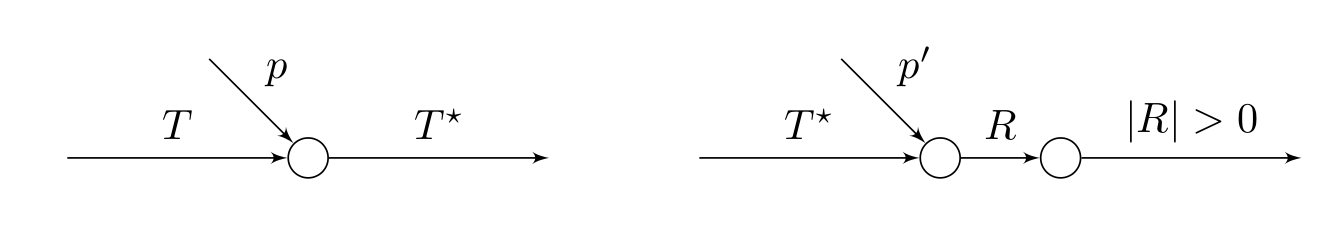
\includegraphics[width=.8\textwidth]{schematic}
\par}

